\documentclass[border=10pt]{standalone}
\usepackage{tikz}
\usetikzlibrary{automata, positioning, arrows.meta}

\begin{document}
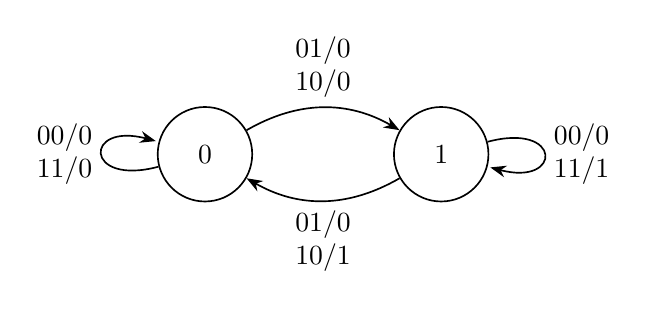
\begin{tikzpicture}[
    ->, >=Stealth, auto, semithick, node distance=3cm,
    state/.style={circle, draw, minimum size=1.2cm, font=\bfseries}
]

    % Nodes
    \node[state] (S0) {$0$};
    \node[state] (S1) [right of=S0] {$1$};

    % Transitions
    % From S0 (A=0)
    % 00 -> 0 (z=0)
    % 11 -> 0 (z=0)
    % 01 -> 1 (z=0)
    % 10 -> 1 (z=0)
    
    \path (S0) edge [loop left] node [align=center] {$00/0$\\$11/0$} (S0)
          (S0) edge [bend left] node [align=center] {$01/0$\\$10/0$} (S1);

    % From S1 (A=1)
    % 00 -> 1 (z=0)
    % 11 -> 1 (z=1)
    % 01 -> 0 (z=0)
    % 10 -> 0 (z=1)

    \path (S1) edge [loop right] node [align=center] {$00/0$\\$11/1$} (S1)
          (S1) edge [bend left] node [align=center] {$01/0$\\$10/1$} (S0);

\end{tikzpicture}
\end{document}
